\documentclass[tikz]{standalone}
\usetikzlibrary{fit, positioning}

\begin{document}
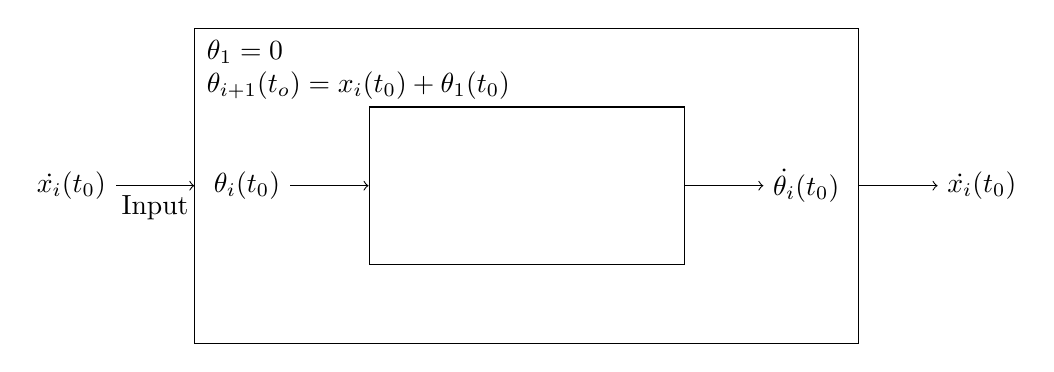
\begin{tikzpicture}
\node[minimum width=4cm, minimum height=2cm, draw] (inner) {};
\draw[->] (inner.east)--++(0:1cm) node[right](thetadot){$\dot{\theta_i}(t_0)$};
\draw[<-] (inner.west)--++(180:1cm) node[left](theta){$\theta_i(t_0)$};
\node[fit=(theta) (thetadot), minimum height=4cm, draw] (outer) {};
\draw[->] (outer.east)--++(0:1cm) node[right] (x-in){$\dot{x_i}(t_0)$};
\draw[<-] (outer.west)-- node[below]{Input} ++(180:1cm) node[left] (x-out){$\dot{x_i}(t_0)$};
\node[below right=1pt and 1pt of outer.north west, align=left]{$\theta_1=0$\\$\theta_{i+1}(t_o)=x_i(t_0)+\theta_1(t_0)$};
\end{tikzpicture}
\end{document}